
\section{Body Axis } \label{sec:body} 
A spacecraft body axis associated with a coordinate system fixed in the body itself at its center of mass. This provides a convenient system to refer the vehicle rotational state.
A favored rotation sequence is  an orientation change is subdivided into three consecutive rotations, first around the $x$-axis with angle roll, followed by a rotation around the $y$-axis with angle pitch, and finally another rotation around the actual $z$-axis with angle yaw. 
In order to illustrate this system we pick an example vehicle system as shown in figure \ref{fig:10}

\textbf{Coordinate Frame:} Non-inertial

\begin{itemize}
\item X-axis: positive toward the vehicle cone apex.
\item Y-axis: Parallel to the Vehicle Structural Coordinate System Y-axis, positive toward the crew's right when the crew is seated facing the cone apex.
\item Z-axis: positive in the direction pointing away from the windows and "down" relative to a seated crew member.
\end{itemize}

\begin{figure}[htp]
\centering
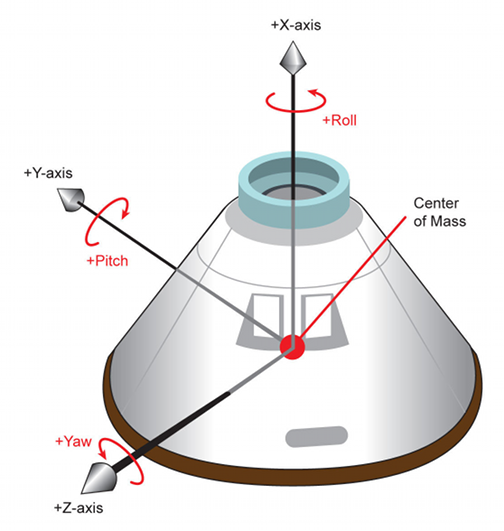
\includegraphics [width=7in]{figs/fig10.png}
\caption{Body Axis}
\label{fig:10}
\end{figure}

\paragraph{Example Body Axis}
See the following JEOD models for an example, \hypermodelref{ORIENTATION} and \hypermodelref{DERIVEDSTATE}.


